\documentclass{article}
\usepackage[utf8]{inputenc}

\usepackage{url}
\usepackage{geometry}
\geometry{
    a4paper,
    left=20mm,
    top=25mm,
    bottom=25mm,
    right=20mm,
 }
 \usepackage{graphicx}
 \usepackage{titling}
 \usepackage{minted}
 \usepackage{amsmath}
 \usepackage{amssymb}
 \usepackage{hyperref}
 \usepackage{xcolor}
 % Color of the university of tübingen
 \definecolor{ekut}{RGB}{165, 30, 55}
 \usepackage[printonlyused,withpage]{acronym} % Acronyms with \ac{NCBI} and \acro{NCBI}{National ...}
 
% Fancy block quotes
\usepackage{mdframed}     
\mdfdefinestyle{bquote}{
    linecolor=gray,
    linewidth=1pt,
    leftmargin=20pt,
    innerleftmargin=5pt,
    leftline=true,
    topline=false,
    bottomline=false,
    rightline=false,
    }
\newcommand{\blockquote}[1]{  \begin{mdframed}[style=bquote]  #1  \end{mdframed}}


% BibLaTex / Biber
\usepackage[backend=biber,
    style=numeric,
    uniquelist=false,
    sorting=none,
    url = true,
    isbn = false,
    giveninits=true,
    uniquename=false,
    maxbibnames=6,
    maxcitenames=2,
    minbibnames=5,
    mincitenames=1,
date=year]{biblatex}
\addbibresource{ref.bib}


% No ident for whole document
\setlength\parindent{0pt}

\title{Layouting Phylogenetic Networks using MIQP}
\author{Jules Kreuer}
\date{\today}
 
\usepackage{fancyhdr}

\renewcommand{\headrule}{\hbox to\headwidth{
\color{ekut}\leaders\hrule height \headrulewidth\hfill}}

\fancypagestyle{plain}{%  the preset of fancyhdr 
    \fancyhf{} % clear all header and footer fields
    \fancyfoot[R]{
\includegraphics[width=2.5cm]{figures/unilogo.pdf}}
    \fancyfoot[C]{\thepage}
    \fancyfoot[L]{December 2022}
    \fancyhead[L]{Layouting Phylogenetic Networks using MIQP}
    \fancyhead[R]{\theauthor}
}
%\pagestyle{plain} % Comment this in if the header / footer should only be on every page.

\makeatletter
\def\@maketitle{%
  \newpage
  \null
  \vskip 1em%
  \begin{center}%
  \let \footnote \thanks
    {\LARGE \@title \par}%
    \vskip 1em%
    %{\large \@date}%
  \end{center}%
  \par
  \vskip 1em}
\makeatother

\usepackage{cmbright}
\begin{document}

\maketitle
\noindent\begin{tabular}{ll}
Author: & Jules Kreuer\\
Contact: & jules.kreuer@uni-tuebingen.de\\
Date of submission: & \today\\
Project available on: & \href{https://github.com/not-a-feature/Layouting-Phylogenetic-Networks-using-MIQP}{Github}
\end{tabular}
\section*{Introduction}
In this technical report, we will discuss the layouting of phylogenetic networks using \ac{MIQP}. Our goal is to create an objective function and constraints that accurately capture the quality of a network and can be optimised to find a visually pleasing layout.  

Proper positioning of nodes in a phylogenetic network is crucial for its readability and overall aesthetic appeal. Incorrect positioning can lead to long hybrid edges spanning across the whole network, making it cluttered and difficult to interpret. 

To layout a phylogenetic network using \ac{MIQP}, one first needs to define constraints that are describing the basic network properties. Furthermore an objective function, which represents the measure of goodness of the network layout is needed. The objective function can be defined based on various criteria, such as the number of crossings, the amount of overlap between branches, or the overall compactness of the network.

Once the objective function has been defined, the optimisation problem can be translated into code where the decision variables are the positions of the nodes in the network. The constraints of the problem can include various layout requirements, such as maintaining a minimum distance between nodes or to avoid overlapping branches.

However, this method does have its limitations, which will be tested and discuss in detail. Overall, our goal is to provide a comprehensive overview of using \ac{MIQP} for visualising phylogenetic networks and its potential advantages and drawbacks.
We will be using \textit{IBM CPLEX 22.1.0} as our solver in combination with the \textit{python 3.10 docplex} module.

\subsection*{Background}
The layout and visualisation of networks is a longstanding problem in the field of graph theory and information visualisation. The goal of such visualisation is to effectively convey the structure and relationships within a network to the viewer, while also making the visualisation aesthetically pleasing \cite{tarawaneh-2012}.  Several heuristics are commonly used, including minimising the number of edges that are crossing, clustering similar nodes or closely related nodes, and maximising edge orthogonality \cite{bennett-2007}. 

Some of these heuristics will be implemented using \ac{ILP} / \ac{MIQP}. 
\ac{ILP} is a type of mathematical optimisation problem that involves finding the values of a set of decision variables that minimise or maximise an objective function, subject to a set of linear constraints. In an \ac{ILP}, all of the decision variables are required to take on integer values, rather than continuous or fractional values. This can make \ac{ILP} problems more challenging to solve, as the solution space is discrete and often larger than for continuous optimisation problems.

A \ac{MIQP} is a type of optimisation problem that combines the features of an \ac{ILP} with those of a \ac{QP}. In a \ac{MIQP}, the objective function and constraints can include both linear and nonlinear terms, allowing for greater modelling flexibility. However, like in an \ac{ILP}, the decision variables in a \ac{MIQP} must take on integer values.

To create an \ac{ILP} or \ac{MIQP} program, one must first define the objective function and constraints. The objective function defines the measure of success for the optimisation, such as minimising cost or maximising profit. The constraints define the limitations or conditions that must be satisfied by the solution.

Once the objective function and constraints are defined, a solver can be used to find the optimal solution. There are various solvers available, such as IBM Ilog CPLEX \cite{ibm-cplex}, Gurobi, and GLPK.

\newpage
\section*{Creating the MIQP}
The are several ways to quantify the visual quality of a phylogenetic network.  For trees, it is as simple as counting the edges that cross. For networks, it is important how cluttered they are or how long hybrid-edges are.

\subsection*{Terminology, Base Constraints and Objective}
A tree is a data structure that consists of nodes organised in a hierarchy. Each node is connected to exactly one parent node by a directed edge and can have zero or more child nodes. In this work, trees are not oriented from top to bottom but rather from left to right. This unusual configuration allows for easier implementation of the constraints.
The left-most node in the tree, which has no parent node, is called the root and is positioned at $x = 0$. The children of a node are placed one step to the right of their parents at $x = p + 1$. For example, the children of the root are at $x = 1$.

After loading a tree from a \ac{GML} file, this positioning can be done by calling the \texttt{auto\_posx()} method othe the \texttt{Graph} object.

This discrete positioning on the x-axis creates layers which will be important later on.

To ensure that a tree has certain basic properties, we add two constraints:
\begin{enumerate}
    \item The y-position of every node must be greater than 0.
    \item No two nodes can have the same position.
\end{enumerate}
This second constraint was reformulated so that the vertical distance between any two nodes in the same layer must be greater than or equal to 1. The reformulation was necessary as the interface does not support "greater than" inequalities.
When edges are added to a tree, resulting in nodes with in-degree $\geq 2$, the resulting structure is no longer a tree, but rather a network. If the solver is able to find a y-positioning of the nodes that satisfies all constraints, it is said to have found a solution. An optimal solution is one that results in a visually pleasing tree or network.

\subsection*{Trees}
\textit{Code of this sub-project can be found in: }\href{https://github.com/not-a-feature/Layouting-Phylogenetic-Networks-using-MIQP/tree/main/01_tree_const}{\texttt{01\_tree\_const}}.\\
The main property of a visually pleasing tree is that its edges do not cross each other. This property can be represented using simple a constraint. For each pair of nodes the following property must hold:
\begin{align}
    N_A < N_B \land C_A < C_B~ ~\lor~~ N_A > N_B \land C_A > C_B \label{form:donotcross}
\end{align} 

With $N_A, N_B$ nodes of a layer, $N_A \neq N_B$ and $C_A, C_B$ a child of $N_A$ and $N_B$ respectively. 
Visualised in figure \ref{fig:crossing} the constraint is only fulfilled in the top two configurations.
\begin{figure}[H]
    \centering
    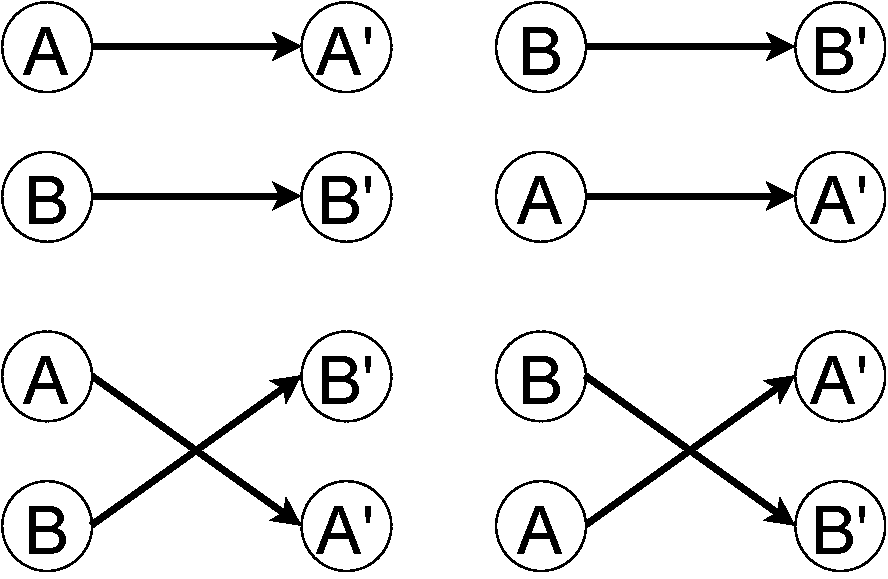
\includegraphics[width=0.25\textwidth]{figures/crossing.pdf} 
    \caption{The 4 possible configurations. Two of them are crossing.}
    \label{fig:crossing}
\end{figure}

Fortunately, CPLEX and its python interface supports logical operations. This constraint represented as code would look like this:
\begin{minted}{python}
model.add_constraint(
    model.logical_or(
        model.logical_and( mvar_node_a <= mvar_node_b, mvar_child_a <= mvar_child_b ),
        model.logical_and( mvar_node_b <= mvar_node_a, mvar_child_b <= mvar_child_a )
    ))    
\end{minted}
Here \texttt{mvar\_node\_a} and \texttt{mvar\_node\_b} are nodes of the same layer with \texttt{mvar\_child\_a} and \texttt{mvar\_child\_b} a children of this nodes respectively.
Using the \texttt{itertools.combinations} package and a nested for loop this constraint is applied on every combination of nodes / children.

However, the time required to solve this problem is highly dependent on the balance of the tree. When the tree is unbalanced, the number of constraints required is small, as there are only a few nodes per layer. When the tree is balanced, the number of constraints required is significantly larger, as it is given by the total number of combinations. As a result, solving the quadratic growing number of constraints for balanced trees is slower.\\
An objective function is added in order to make the trees not only free of edge crossings but also visually pleasing. The function aims to position the parents as close to the centre of their children as possible.

In an effort to reduce the solving time, we implemented two constraints that aimed to limit the search space to a more feasible size:
\begin{enumerate}
    \item Maximum height for every node
    \item A maximum vertical distance between a parent and its child node.
\end{enumerate}
To evaluate the effectiveness of these constraints, we measured the time to solve 200 random trees. Our results showed that both a lower and upper bound on the search space had a slight positive effect on reducing the average time and scatter. However, the second constraint had a negative impact on solving time. This was observed for both balanced and unbalanced trees. A detailed view can be found in figure \ref{fig:01_gridsearch}.

To evaluate the capabilities of this constraint enriched \ac{ILP} approach, we attempted to solve 1000 randomly generated trees ranging in size from 3 to 42. A maximum solving time of 20 seconds was imposed. The impact of balanced trees on the performance of the algorithm is depicted in figure \ref{fig:runtime-tree}.
While almost every unbalanced tree up to 42 nodes was solved in less than a second, CPLEX started to struggle with balanced trees of size 21. Here the time increased and reached the cut-off of 20s.
\begin{figure}[H]
    \centering
    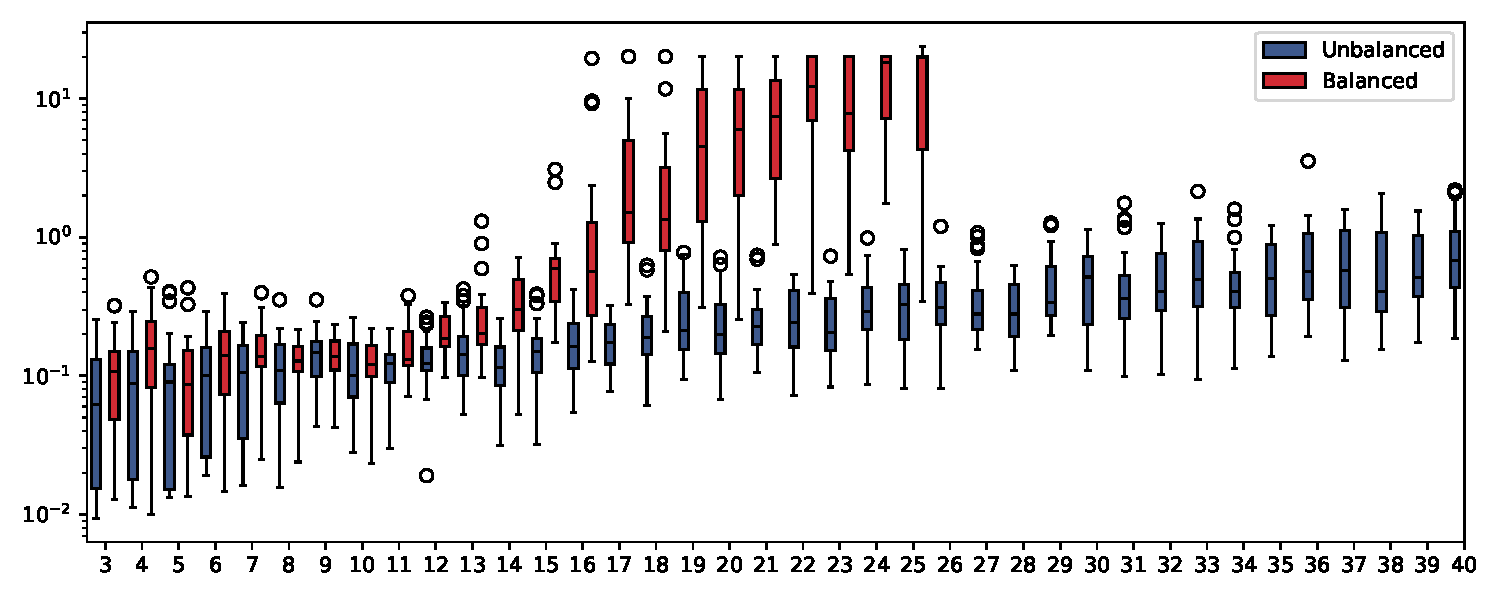
\includegraphics[width=0.8\textwidth]{figures/01_perf.pdf}
    \caption{Time to solve trees of size n (x-axis) in seconds (y-axis, log-scale).}
    \label{fig:runtime-tree}
\end{figure}
\section*{Extensions of Trees}
In this section, we will extend standard trees with additional edges, and subsequently, generate modified constraints and an objective function.

\subsection*{Horizontal Gene Transfer}
\textit{Code of this sub-project can be found in: }\href{https://github.com/not-a-feature/Layouting-Phylogenetic-Networks-using-MIQP/tree/main/02_horiz_embedding_obj}{\texttt{02\_horiz\_embedding\_obj}}.\\
In order to simulate horizontal gene transfer, edges are added to a tree such that they only connect nodes within the same layer. The goal of the objective is to find a configuration where nodes that share a hybrid edge are close. Other tree visualisation algorithms achieve this by flipping subtrees recursively in order to find the optimal position. In our case, the objective is to minimise the square of the length of the hybrid-edges.

It is expected that the solver will be able to find a solution quickly, as the constraints of the problem are not affected by the addition of hybrid edges. However, it is possible that it may take some time to find the optimal solution.

Similarly to the previous section, 1000 balanced and unbalanced trees were generated. A performance overview can be found in the appendix \ref{fig:runtime-horiz-hybrid}.
\begin{figure}[H]
    \centering
    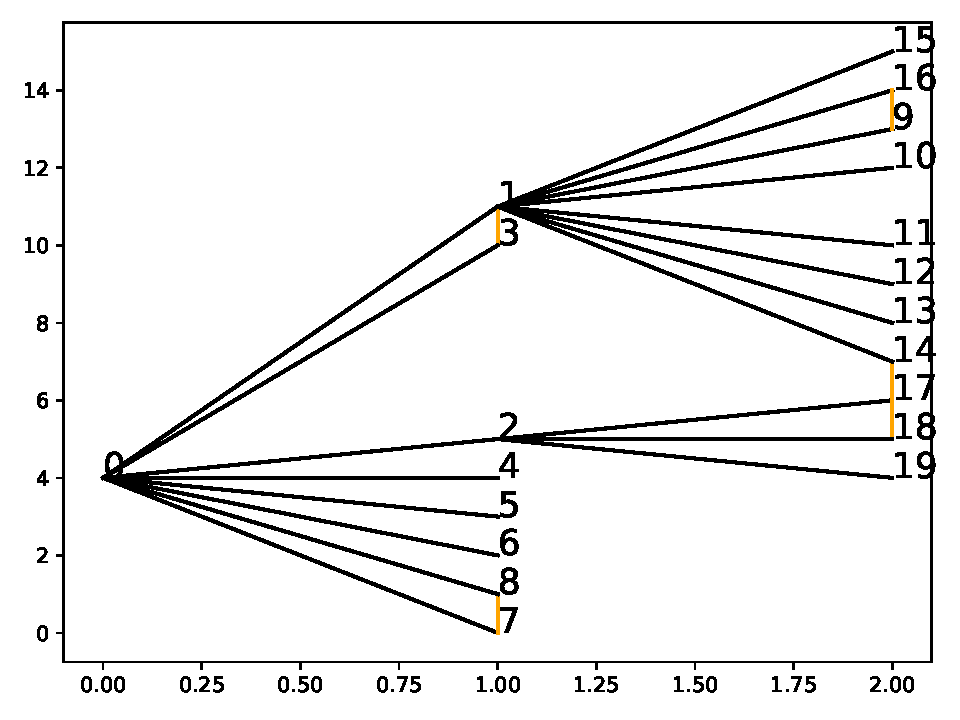
\includegraphics[width=0.3\textwidth]{figures/hybrid_example.pdf} ~ 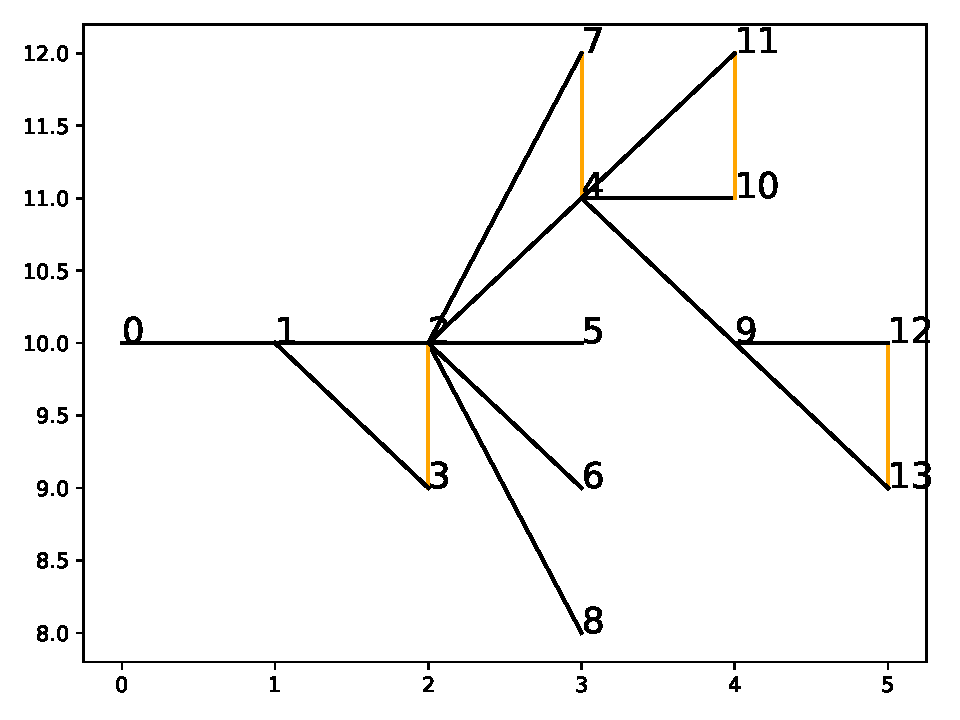
\includegraphics[width=0.3\textwidth]{figures/hybrid_example_2.pdf}
    \caption{Example of an balanced and unbalanced tree with hybrid edges inside one layer.} 
    \label{fig:hybrid-example-horiz}
\end{figure}
Observations have shown that unbalanced trees with hybrid edges are solved effectively. Example trees are shown in figure \ref{fig:hybrid-example-horiz} However, for balanced trees, the same problems that exist without hybrid edges may persist. This is particularly true for larger (size $\geq 20$) problems, where the solutions obtained may not be optimal. Overall, the efficiency and effectiveness of the solver in finding solutions for tree structures with hybrid edges may depend on the balance of the tree and the size of the problem.


\subsection*{Hybrids from n to n+1}
\textit{Code of this sub-project can be found in: }\href{https://github.com/not-a-feature/Layouting-Phylogenetic-Networks-using-MIQP/tree/main/03_hybrid_embedding_obj}{\texttt{03\_hybrid\_embedding\_obj}}.\\
To the previous tree structure, additional edges were added from layer n to n+1. Having a total of three edge types (regular, horizontal, n to n+1), the previously mentioned constraints were only applied to the tree backbone with its regular edges. The hybrid edges are ignored entirely.

To optimise the tree structure, the objective function was extended with the goal of minimising the number of crossings. While this initially seemed like a good idea, there were several difficulties in implementing this objective. Specifically, it was not possible to include control-flow elements like "if/else". As a result, a workaround was developed using only max/abs functions:

\begin{align}
    low(a, b) &= max((b - a) - |b-a|  ,~ -1)\\
    q1 &= low(\text{N}_a, \text{N}_b) + low(\text{C}_a, \text{C}_b)\\
    q2 & = | (low(\text{N}_b, \text{N}_a) + low(\text{C}_b, \text{C}_a) |\\
    obj &= \left(\frac{|q1 + q2|}{2} - 1\right)^2
\end{align}

The function \texttt{low(a,b)}, defined on the set of integers $\mathbb{Z}$, returns $0$ if $a < b$ and $-1$ otherwise. If the edge connecting $\text{N}_a$ to $\text{C}_a$ crosses the edge connecting $\text{N}_b$ to $\text{C}_b$, then the variable $\texttt{obj}$ is equal to $1$. Otherwise, if the edges do not cross, $\texttt{obj}$ is equal to $0$.\\

This objective is applied only on hybrid edges due to its computationally demanding nature. While the solver is able to effectively minimise the crossing using this objective, the maximum number of nodes is limited to around 20 for both balanced and unbalanced trees. The performance of this single objective can be observed in the figure \ref{fig:min_direct_crossing} provided, where the objective \texttt{min\_direct\_crossing} is turned off and on exclusively.

The results indicate that the best outcome is achieved when the computational heavy objective is turned off. It took a total of 3.31 seconds to solve this network. 
The same result was computed when the objective \texttt{min\_direct\_crossing} was turned on and other objectives like the minimisation of hybrid length were active as well. Here the computation took 20 seconds. 
This may be due to the difficulty in optimising objectives with step-like properties (crossing: 1, not crossing 0) and the solver being designed to solve continuous functions. This problem of a "large objective shift" is also recognised during the solving process when such jump is made.\\\\
The performance of multiple trees was tested, and the results were depicted in the following graphs. It is evident from the graphs and the produced trees that the implementation of the \texttt{min\_direct\_crossing} objective increased the complexity for the solver.
\begin{figure}[H]
    \centering
    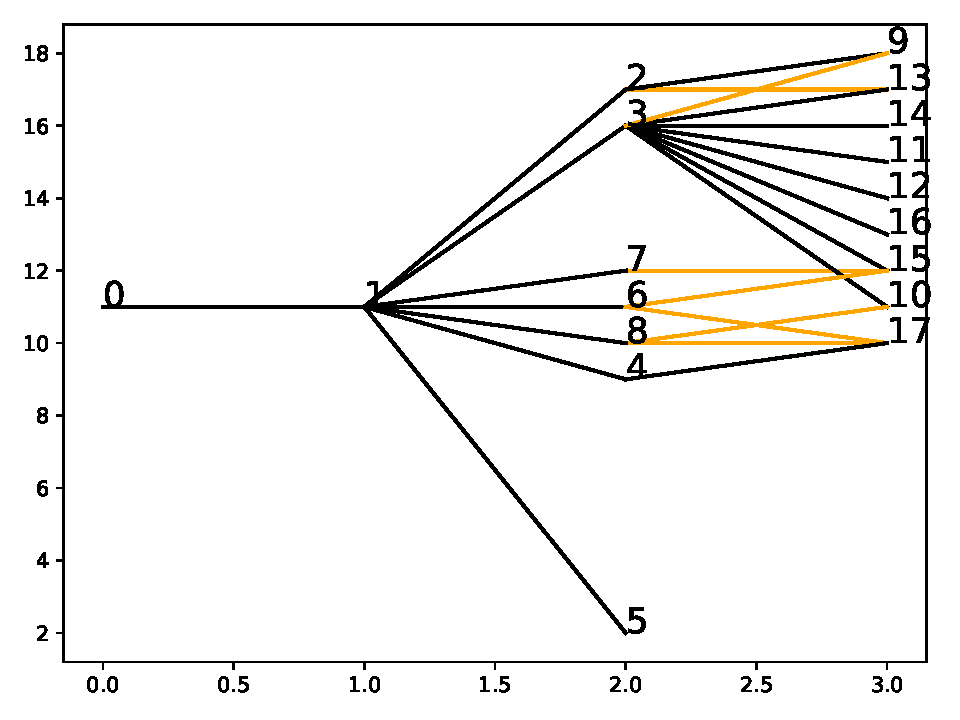
\includegraphics[width=0.3\textwidth]{figures/min_direct_crossing_off.pdf} ~ 
    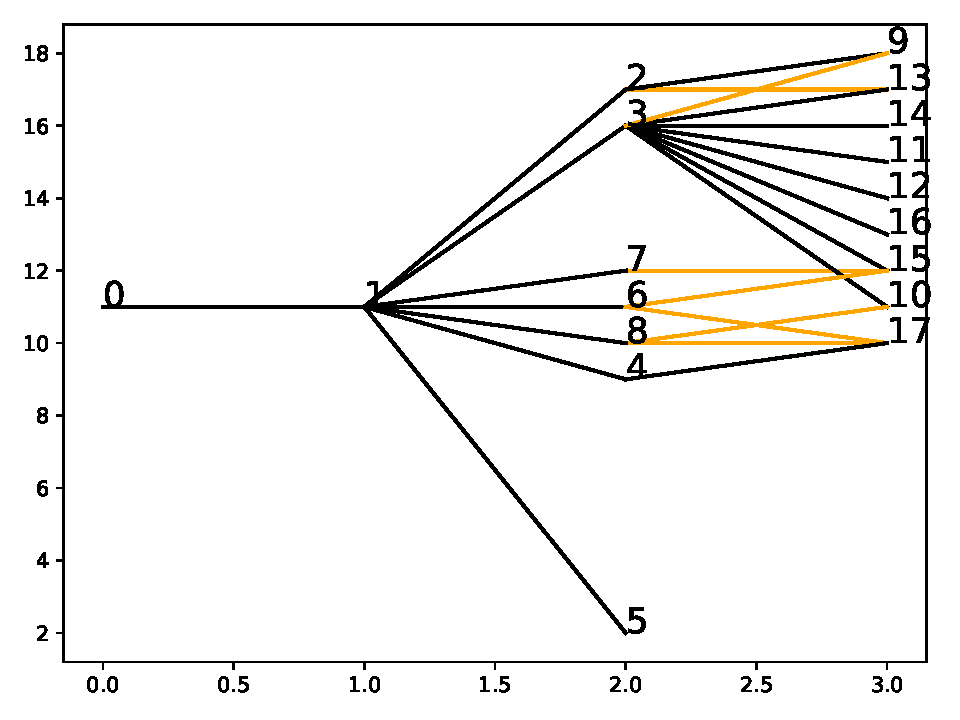
\includegraphics[width=0.3\textwidth]{figures/min_direct_crossing_off.pdf} ~ 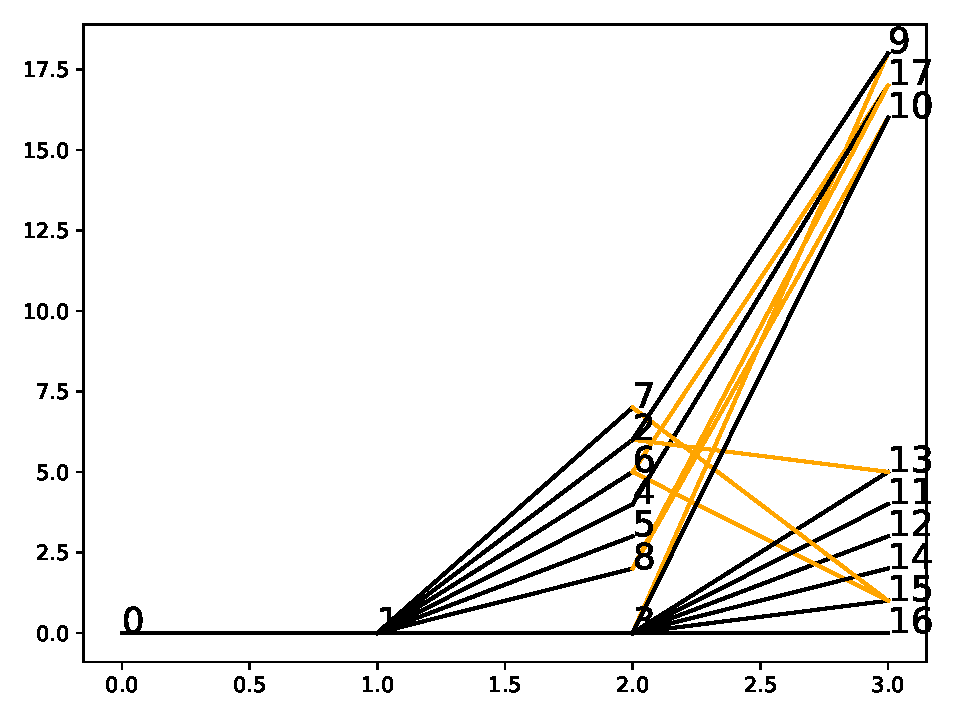
\includegraphics[width=0.3\textwidth]{figures/min_direct_crossing_only.pdf}
    \caption{\textbf{Left}: \texttt{min\_direct\_crossing} tuned off. Other objectives turned on. The best possible positioning (4 crossings) was found in 3.31s. \textbf{Centre}: \texttt{min\_direct\_crossing} tuned on. Other objectives turned on.  \textbf{Right}: Only \texttt{min\_direct\_crossing} active. Time-limit of 20s reached.}
    \label{fig:min_direct_crossing}
\end{figure}

\begin{figure}[H]
    \centering
    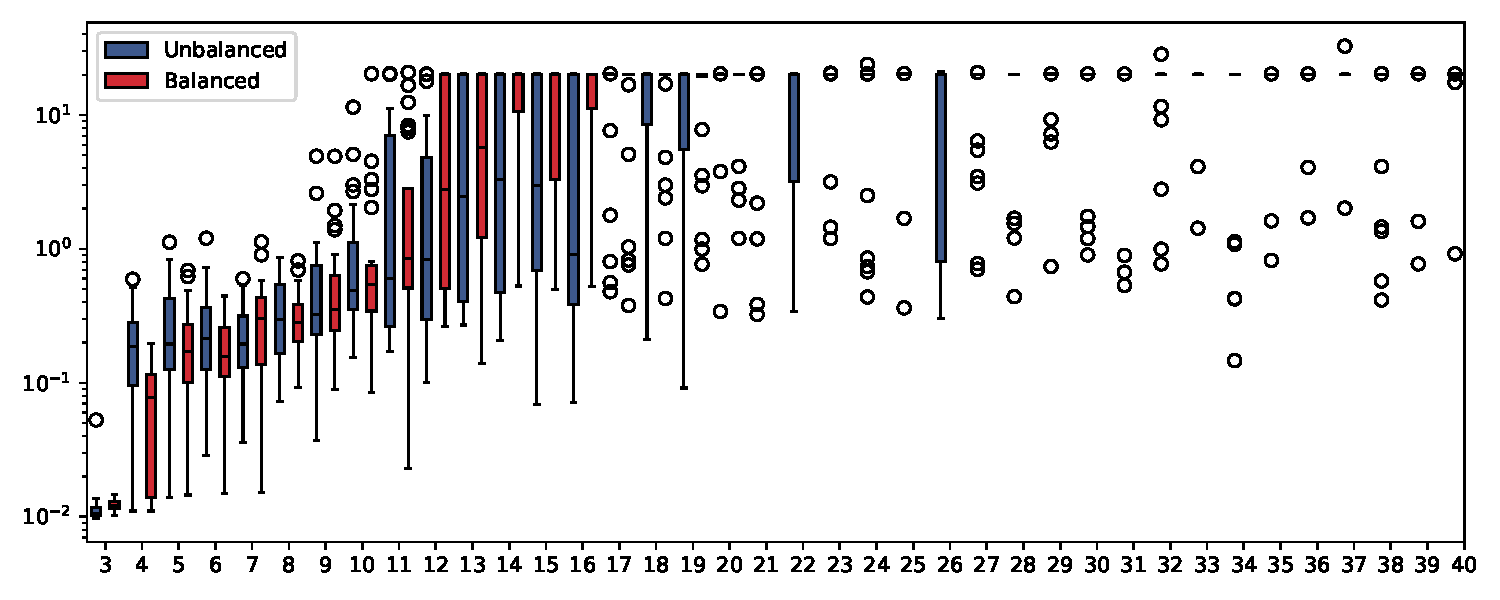
\includegraphics[width=0.8\textwidth]{figures/03_perf_min_crossing.pdf}\\
    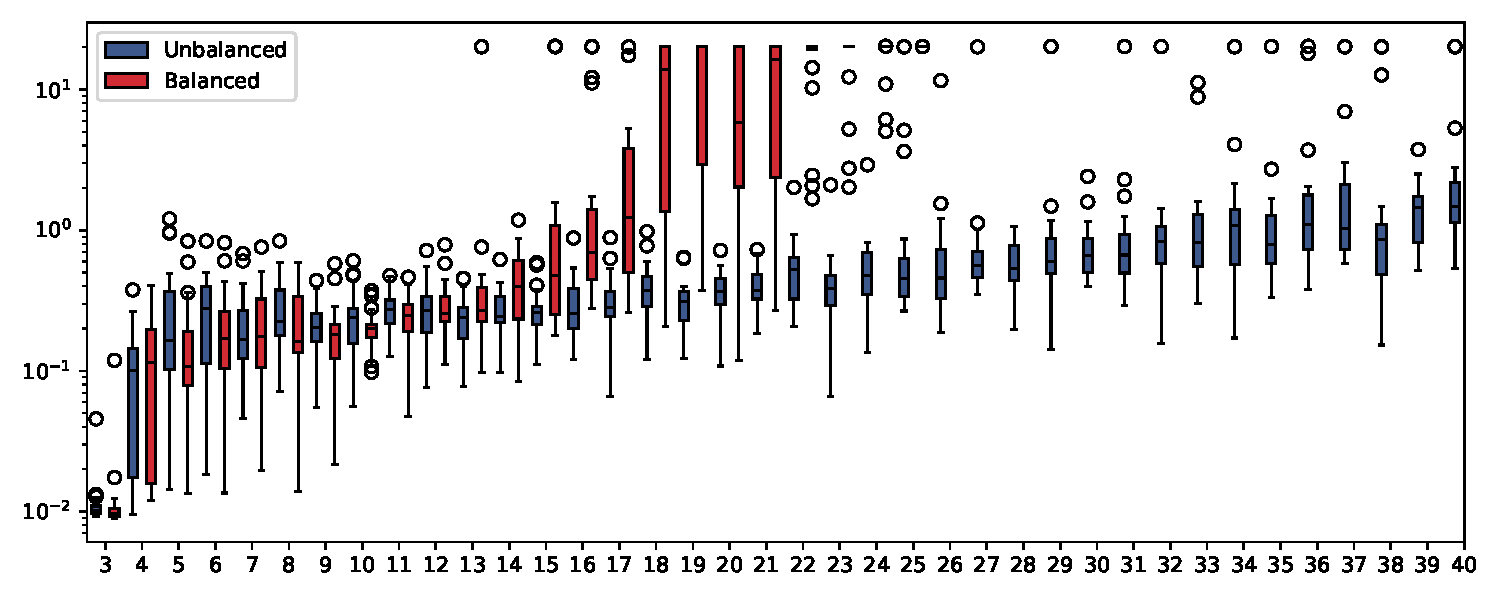
\includegraphics[width=0.8\textwidth]{figures/03_perf_without.pdf}\\
    \caption{Time to solve trees of size n (x-axis) in seconds (y-axis, log-scale). \textbf{Top}: \texttt{min\_direct\_crossing} tuned on. \textbf{Bottom}: \texttt{min\_direct\_crossing} tuned off.}
    \label{fig:runtime-tree}
\end{figure}
\newpage
\subsection*{Multi-layer hybrids}
\textit{Code of this sub-project can be found in: }\href{https://github.com/not-a-feature/Layouting-Phylogenetic-Networks-using-MIQP/tree/main/04_mult_embedding_obj}{\texttt{04\_multi\_embedding\_obj}}.\\
As part of the investigation into the capabilities of using \ac{MIQP} on increasingly complex structures, the next step is to allow for the use of hybrid edges in general, rather than just between adjacent layers (x to x+1).\\\\

To avoid the need for modifying the objective function, a method from the Sugiyama algorithm is employed \cite{sugiyama}. This involves introducing dummy nodes with in-degree and out-degree of one into edges that span multiple layers, effectively converting the trees into those described in the previous section. Upon completion of the optimisation, these dummy nodes are removed.
\begin{figure}[H]
    \centering
    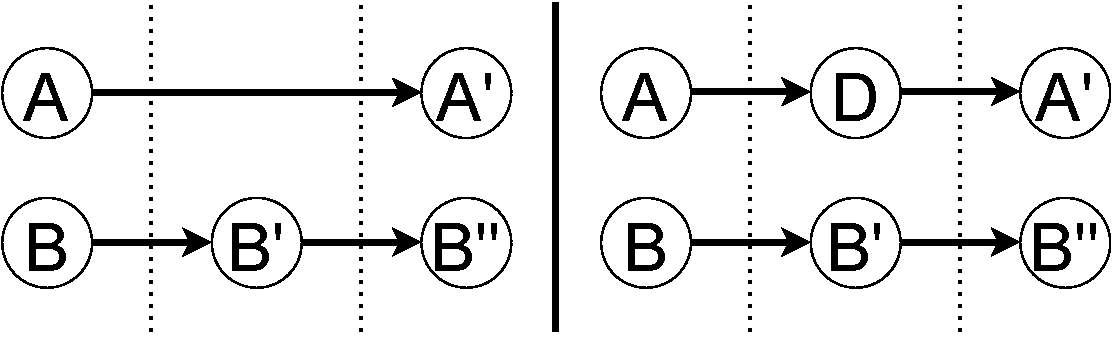
\includegraphics[width=6cm]{figures/dummy_nodes.pdf}
    \caption{The dummy node \texttt{D} is inserted into the edge from \texttt{A} to \texttt{A'}}
    \label{fig:dummy}
\end{figure}

Similar results were observed due to the similarities with the previous problem. However, as there were slightly more nodes present in these problems, the time limit of 20 seconds was reached slightly earlier (see figure \ref{fig:runtime-multi-hybrid}).
We found that the objective function used did not adequately capture the quality of the trees. Specifically, we observed that long hybrid edges were crossing other edges, which was largely due to the objective of minimising the vertical hybrid edge length. This resulted in horizontal edges (vertical length = 0), but did not check for possible crossings. An example of such crossing can be found in figure \ref{fig:long_edges}
\begin{figure}[H]
    \centering
    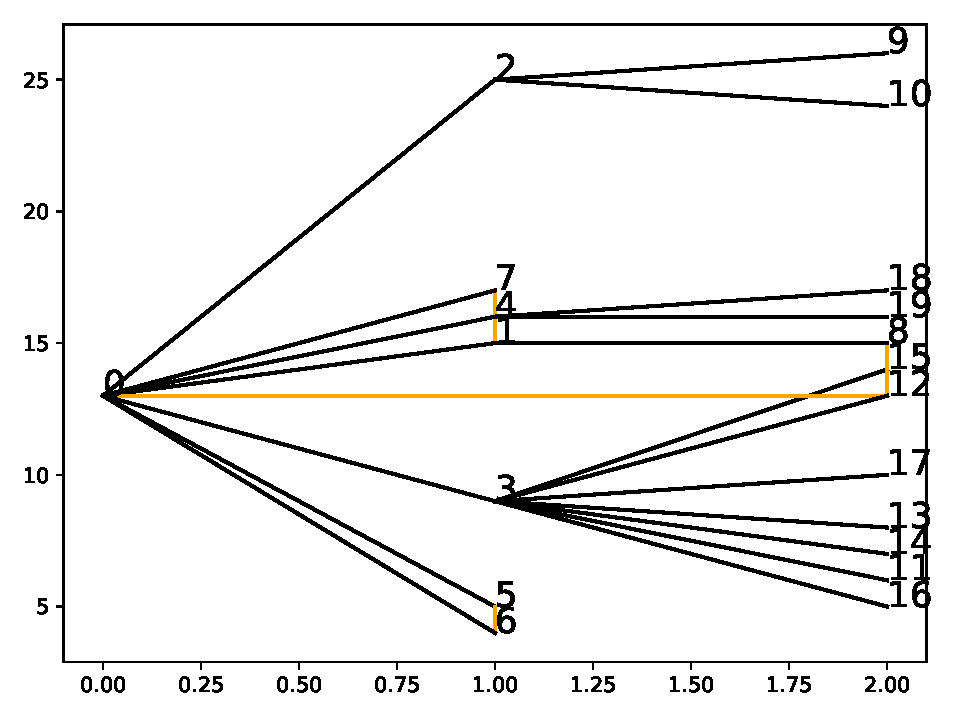
\includegraphics[width=0.3\textwidth]{figures/long_edge.pdf} ~
    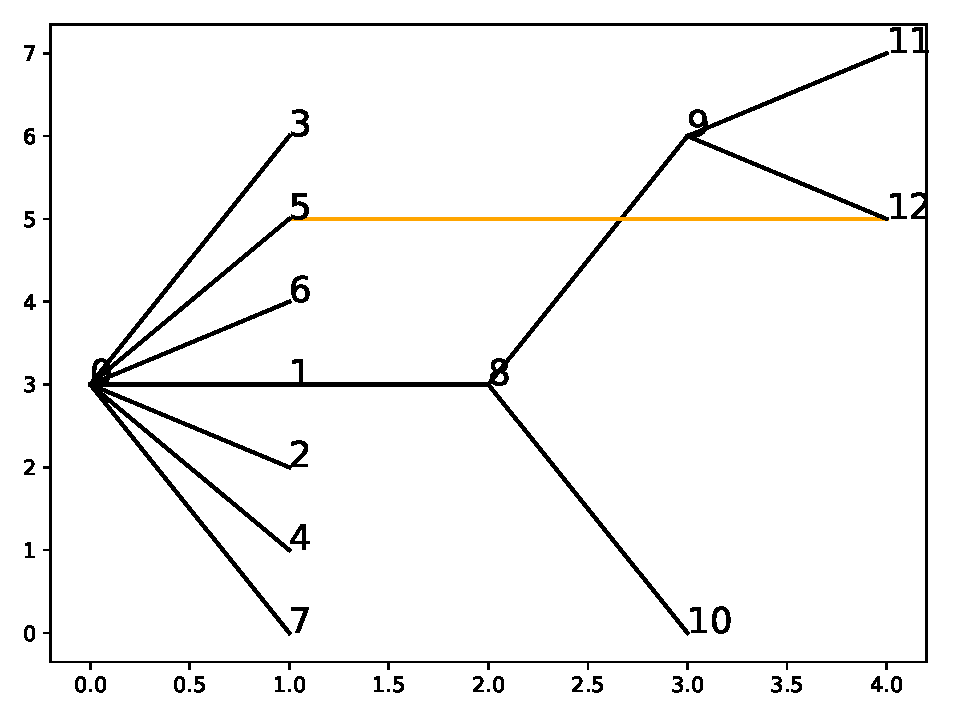
\includegraphics[width=0.3\textwidth]{figures/long_edge_2.pdf}
    \caption{Long hybrid edges are crossing other edges even though the global minimum of the objective function was found.} 
    \label{fig:long_edges}
\end{figure}

One possible solution to this issue is only applying this objective to hybrid edges within the same layer. However, we also explored the use of additional objectives to improve the results, but none were found to be effective.
\newpage
\section*{Networks Heuristic}
\textit{Code of this sub-project can be found in: }\href{https://github.com/not-a-feature/Layouting-Phylogenetic-Networks-using-MIQP/tree/main/05_network_heuristic}{\texttt{05\_network\_heuristic}}.\\
In the context of full phylogenetic networks, it can be challenging to identify which edges are hybrid edges. As a result, if a node has multiple parents, each of those edges is considered a hybrid edge. This leads to a sparse tree embedding, which reduces the effectiveness of the previously used tree constraints.

Direct optimisation through the minimisation of crossings has been demonstrated to be slow. As an alternative, an attempt was made to approximate the solution using multiple heuristic objectives. A total of six objectives were used: 
Nodes with the same parent (i.e. siblings) should be positioned as closely as possible. This can be achieved by minimising the pairwise distance between these nodes, resulting in the formation of groups. The parent node of each group should be centred within the group. This is sufficient to solve regular trees and find a positioning without edge crossings.
To reduce the clutter of the network, the distance between groups should be maximised. These three objectives are visualised on the left side of figure \ref{fig:objective}.

To improve the placements of hybrid edges, the \ac{LCSA} is determined for each node with multiple parents. The \ac{LCSA} is the rightmost node that is an ancestor of all the parents of the node in question. The vertical distance between the node and the \ac{LCSA} is minimised.  This should position the node in between the multiple paths to its \ac{LCSA}. Additionally, similar to the approach described in the previous section, the vertical length of hybrid edges is minimised. These objectives are visualised on the right-hand side of figure \ref{fig:objective}.
\begin{figure}[H]
    \centering
    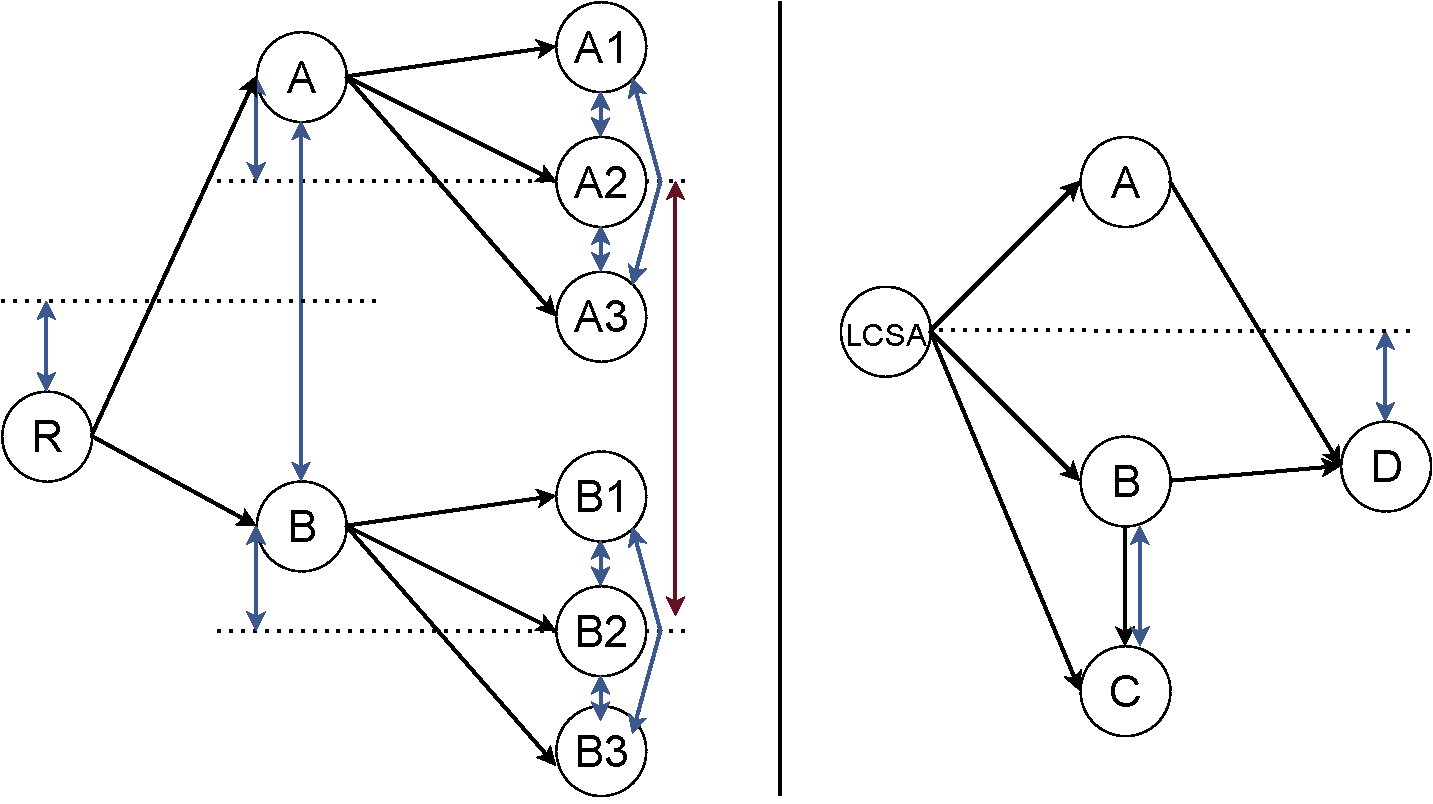
\includegraphics[width=0.6\textwidth]{figures/objective.pdf}
    \caption{\textbf{Left}: Visualisation of the three first objectives. \textbf{Right}: Visualisation of two last objectives. The distance indicated by the blue arrows should be minimised. The red arrow maximised.}
    \label{fig:objective}
\end{figure}
We found that the resulting trees were often not visually pleasing. In many cases, horizontal edges spanning multiple layers were crossing other edges. Turning the \texttt{min\_hybrid\_length} objective off solved that issue but introduces more crossing in other networks. 
Even for unbalanced trees with sizes greater than 20, the time limit was frequently reached before a satisfactory solution could be found (visualised in figure \ref{fig:runtime-network}).
This suggests that the chosen objective is not well-suited for producing high-quality layouts of larger phylogenetic networks.

\newpage
\section*{Understanding the optimisation process}
The solving process is highly dependent on the solver used. In this case, CPLEX by IBM ILOG is utilised \cite{ibm-cplex}.

Several factors can impact the solving process, including the search space, the satisfiability of the constraints, the computational complexity of the objective function, the search strategy and the optimality criterion.

As demonstrated in \ref{fig:01_gridsearch}, restricting the search space through the use of upper and lower bounds on the positions of all nodes can reduce the runtime as well as the scatter. This is because the search space is limited to a smaller region. However, if the upper and lower bounds are set too closely, it may become impossible to find a solution.\\

The given constraints are creating a so-called \ac{SAT} problem where the goal is to find a solution that satisfies this set of constraints. When solving a tree, the main constraint was that edges should not cross \ref{form:donotcross}. CPLEX is able to solve those \ac{SAT} problems efficiently as shown in \ref{fig:runtime-tree} by using techniques like branch-and-cut \cite{ibm-what} \cite{ibm-solve}.\\

The computational complexity of the objective function can also impact the speed at which a problem can be solved. If the objective function is large and difficult to compute, it slows down the solving process, as it must be recalculated for each potential solution that is explored. Furthermore, if the objective function contains functions that map multiple values to a single result (e.g., the absolute value function or the square function), the solver may need to explore both directions in order to determine the optimal solution. This can further increase the computational complexity. The presence of non-continuous functions, such as the count of crossing edges, also poses a challenge for solvers like CPLEX. As these functions do not have a gradient and will lead to a sudden shift of the objective, gradient-based algorithms such as simplex aren't that effective.\\

CPLEX employs two primary solving strategies: branch-and-cut and dynamic search \cite{ibm-dynsearch}. If no specific strategy is specified, CPLEX will automatically choose the most appropriate one based on the characteristics of the problem. For the problems presented in this work, dynamic search is often the preferred method.
Following the dynamic search strategy, CPLEX solves a series of continuous sub-problems. To manage these sub-problems efficiently, CPLEX constructs a tree in which each sub-problem is represented as a node. The root of the tree is the continuous relaxation of the original \ac{MIQP} problem.\\

If the solution to the relaxation includes one or more fractional variables, CPLEX attempts to identify and add cuts, which are constraints that eliminate areas of the feasible region of the relaxation that contain fractional solutions. CPLEX can generate various local cuts that affect only a subtree, as well as global cuts affecting the whole problem.\\

If the relaxation solution still includes fractional-valued integer variables after the addition of cuts, CPLEX branches on a fractional variable, creating two new sub-problems with more restrictive bounds on the branching variable. For example, with binary variables, one node will fix the variable at 0, while the other fixes it at 1. If the sub-problems result in a fractional solution, the process is repeated. If the solution is infeasible or all-integer, the branch-and-cut algorithm terminates.\\

Determining when to stop the search is an important consideration in this \ac{MIQP} optimisation.

CPLEX terminates under a number of conditions \cite{ibm-terminating}. The most significant of these is the time limit set by the user. Additionally, CPLEX may declare integer optimality and terminate the search if it finds an integer solution and has found the global optimum. However, this scenario is only likely to occur for small or unbalanced trees, as it requires all parts of the search space to be searched. In the default mode, "balance optimality and feasibility," CPLEX uses tactics that aim to find a proven optimal solution quickly for a wide range of problem difficulties \cite{ibm-performance}. The branching strategy is designed to find high-quality feasible solutions without sacrificing too much time that could be spent proving the optimality of any solutions that have already been found.
An alternate mode, "focus on feasibility," puts less emphasis on analysis and proof of optimality. As this mode was not selected, it could be the subject of further research.\\

It is interesting to examine the process of the solving steps and how the solution evolves over time. In the next figure \ref{fig:network_process}, we visualise some intermediate results of one optimisation attempt.
\begin{figure}[H]
    \centering
    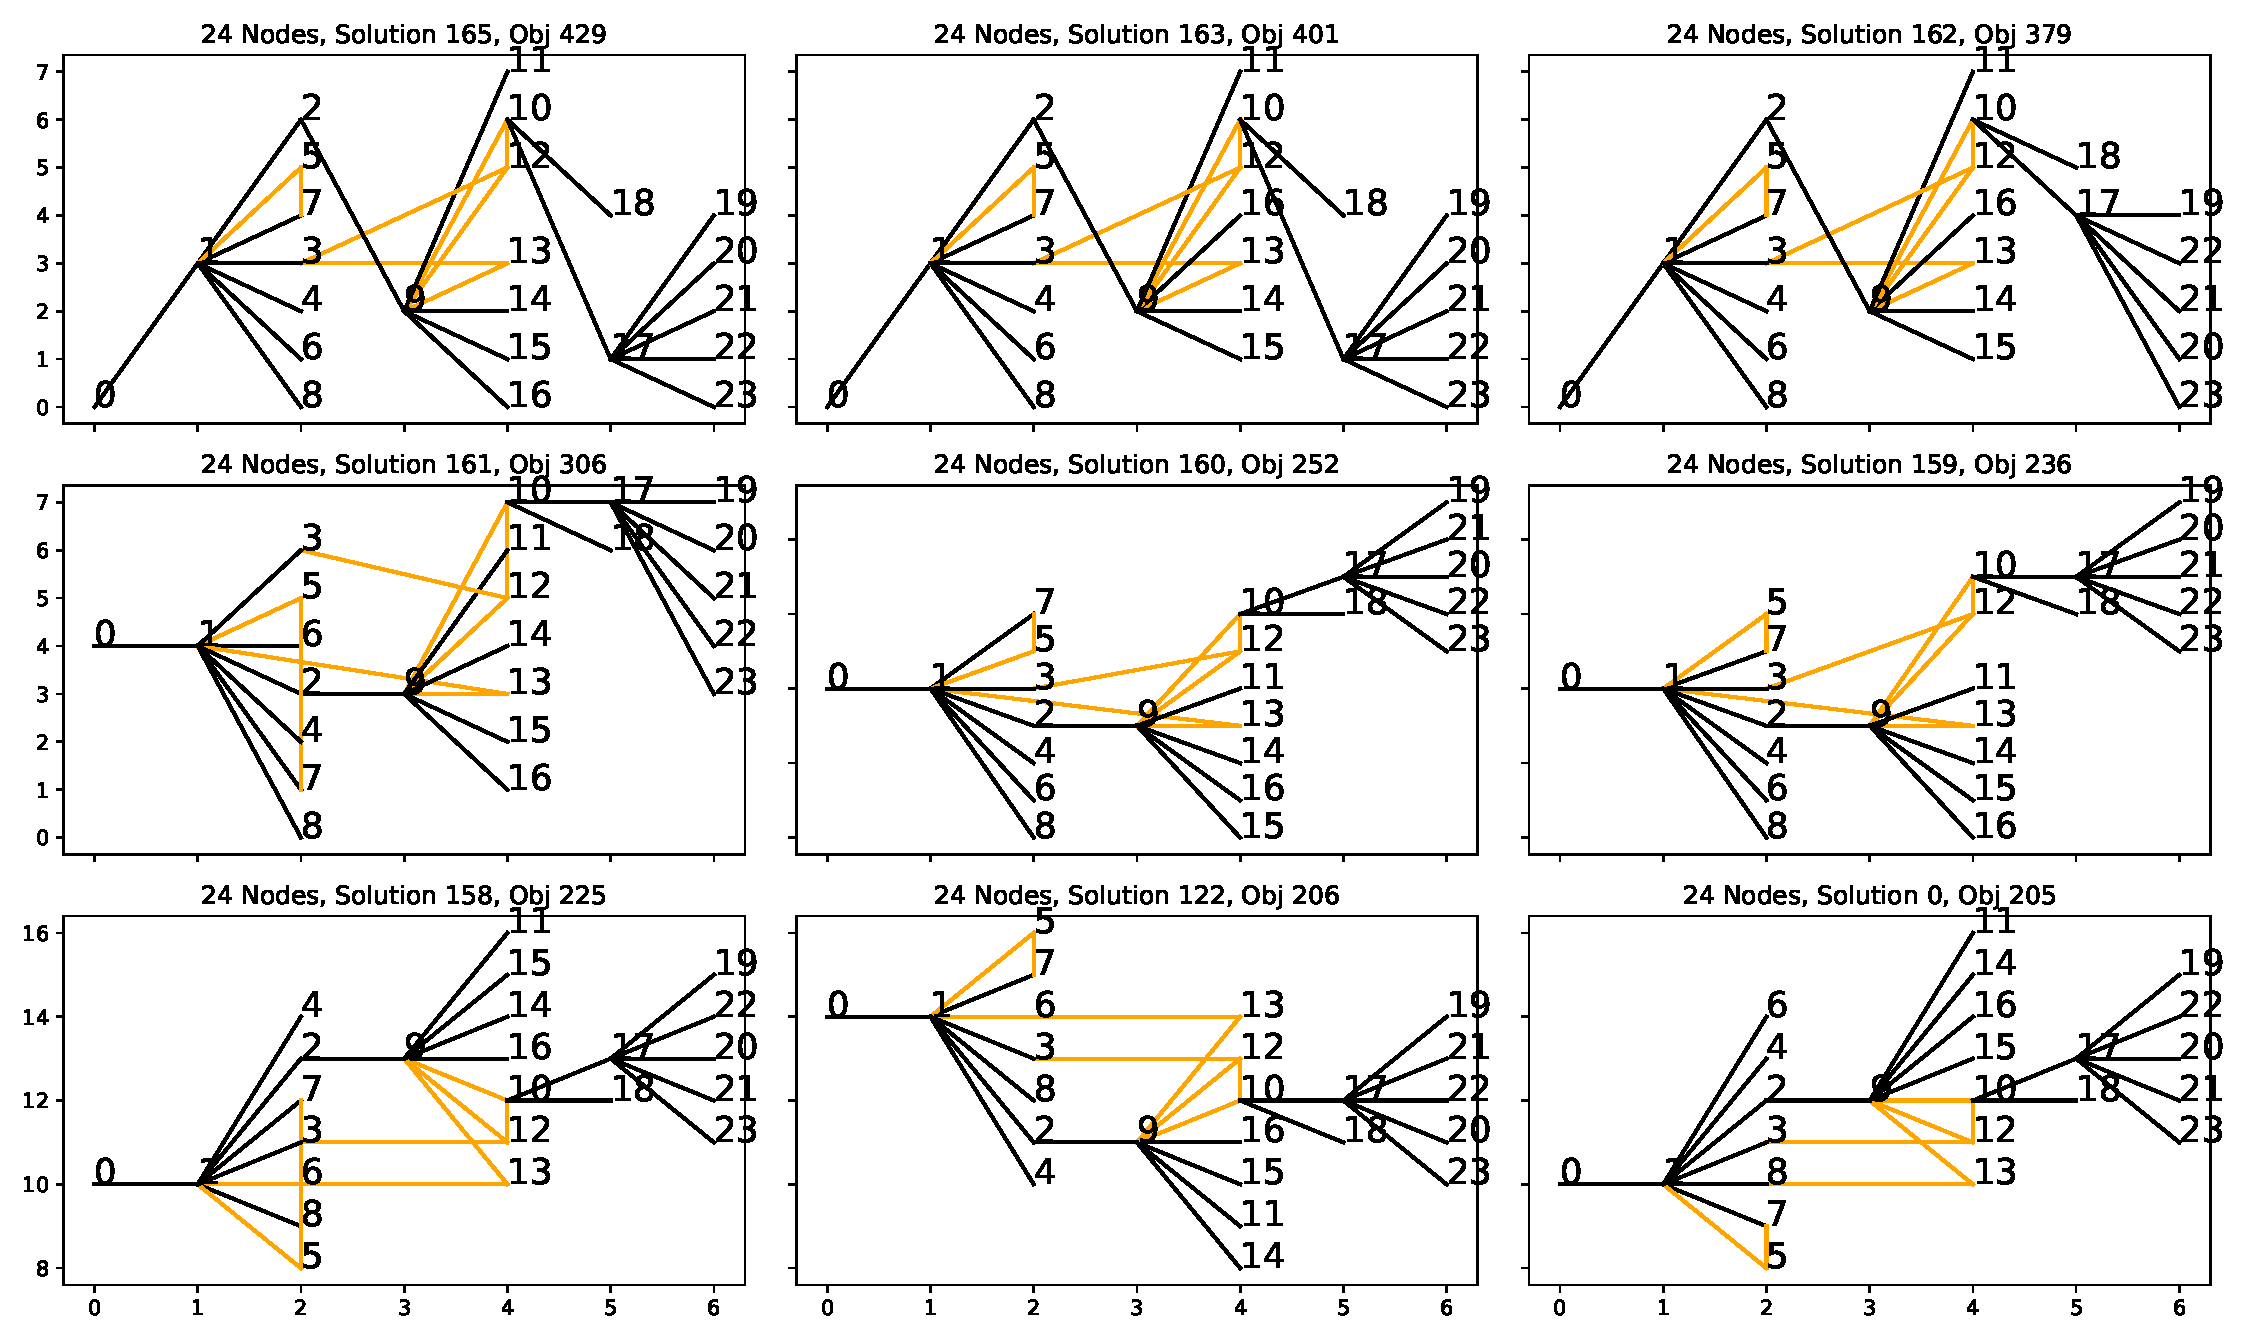
\includegraphics[width=0.8\textwidth]{figures/network_process.pdf}
    \caption{Intermediate solutions while solving a network. The objective score ranges from 429 to 205.}
    \label{fig:network_process}
\end{figure}

The first solution (top left) satisfies all constraints, but it is far from optimal. For example, it is clear that the objective of having parents centred between their children has not been fully optimised yet, as evidenced by the position of node 10 and its children 17 and 18. However, over the next solutions, it is clear that the children are being positioned more closely to one another.

Overall, the objective function values decrease from 429 for the first solution to 205 for the final solution, indicating that the solution is improving over time. Examining the intermediate results can provide insight into the optimisation process and help to identify areas for further improvement.

\section*{Summary and further research}
In this work, we explored the use of mixed integer quadratic programming (\ac{MIQP}) to lay out nodes in phylogenetic trees and networks.

We were able to formulate constraints to describe trees and successfully solve all types of them, including large, balanced, and unbalanced ones. However, as the complexity of the problem increased when applied to networks, we observed diminishing returns. Tree-embedded networks with horizontal hybrids were still solvable and produced high-quality trees. This was achieved by minimising the length of the hybrid edges. More complex structures like trees with hybrid edges spanning across multiple layers became very difficult to solve. In this case, only unbalanced trees produced visually pleasing results, likely due to the quadratic growth of constraints in balanced trees.

We also found that directly minimising the number of crossings was slow. This is due to the high computational cost and step-like properties of the objective. When no information about tree embeddings was available, we had to approximate the qualities of a readable network using multiple objective functions. This approach provided acceptable results for simple or small networks, but for larger ones (size $\geq 20$), it was practically infeasible. For most smaller networks, it was possible to find a combination objectives that resulted in good results, but none was found that was applicable to all networks.

In conclusion, we can say that the use of \ac{MIQP} to layout nodes in phylogenetic trees and networks may not be the most effective approach as already other good heuristics are available. However, there are still many avenues that could be explored, such as the use of different solvers or solving strategies, or the incorporation of alternative objectives that may lead to better results.


\newpage
\section*{List of Abbreviations}
\begin{acronym}[MIQP-] % laengste kurzform hier einsetzen
\setlength{\parskip}{0ex}
\setlength{\itemsep}{0ex}
\acro{GML}{Graph Markup Language}
\acro{ILP}{Integer Linear Programming}
\acro{LCSA}{Last Common Stable Ancestor}
\acro{MIQP}{Mixed-Integer Quadratic Programming}
\acro{QP}{Quadratic Programm}
\acro{SAT}{satisfiability}
\end{acronym}

\section*{Appendix}
\subsubsection*{Code and Data}
The complete code used, the complete data produced and every plot for this project can be found at:\\\url{https://github.com/not-a-feature/Layouting-Phylogenetic-Networks-using-MIQP}.

\subsubsection*{System Specifications}
The system on which the runtime and speed were tested was a Framework Laptop with the following specifications:
\begin{itemize}
    \item Device: Framework Laptop DIY Edition
    \item CPU: Intel i5-1240P (Up to 4.4 GHz, 4+8 cores)
    \item Memory: 16GB (1 x 16GB) DDR4-3200
    \item System: Linux Mint 21 Vanessa 
    \item Kernel: 5.15.0-56-generic
\end{itemize}

\subsubsection*{Software Specifications}
The following packages were used:
\begin{itemize}
    \item IBM ILOG CPLEX Optimization Studio 22.1.0.0 \cite{ibm-cplex}
    \item matplotlib 3.5.2 \cite{matplotlib}
    \item numpy 1.23.1 \cite{numpy}
    \item python 3.10.4 \cite{python}
\end{itemize}
A complete conda environment can be found in file \href{https://github.com/not-a-feature/Layouting-Phylogenetic-Networks-using-MIQP/blob/main/enviroment.yml}{\texttt{enviroment.yml}}
\newpage
\subsubsection*{Additional figures}
 \begin{figure}[H]
     \centering
     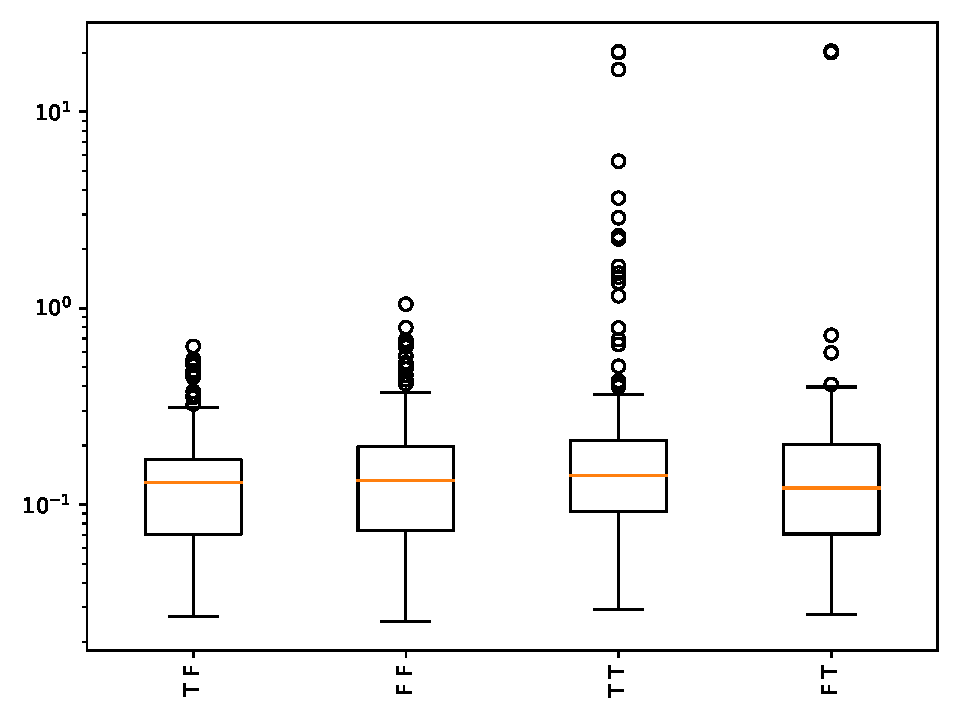
\includegraphics[width=0.5\textwidth]{figures/01_grid.pdf}
     \caption{Time to solve trees using different constraints. Each run is repeated with 200 balanced trees with 7 - 15 nodes. First constraint is \texttt{max\_height\_by\_nodes}, second one \texttt{c\_withing\_range}. An active constraint is represented with a \texttt{T}, an inactive one with a \texttt{F}.}
     \label{fig:01_gridsearch}
 \end{figure}

 \begin{figure}[H]
    \centering
    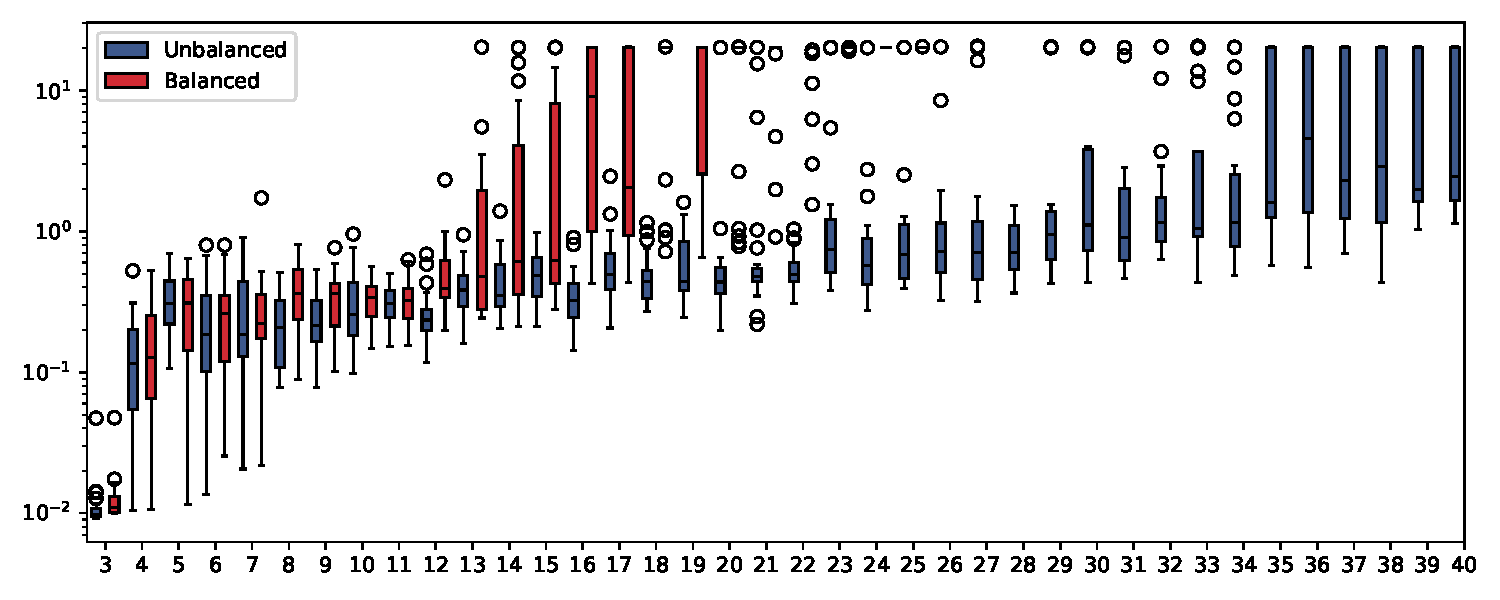
\includegraphics[width=0.8\textwidth]{figures/02_perf.pdf}
    \caption{Time to solve trees of size n (x-axis) with hybrid edges inside the same layer. In seconds (y-axis, log-scale).}
    \label{fig:runtime-horiz-hybrid}
\end{figure}

 \begin{figure}[H]
    \centering
    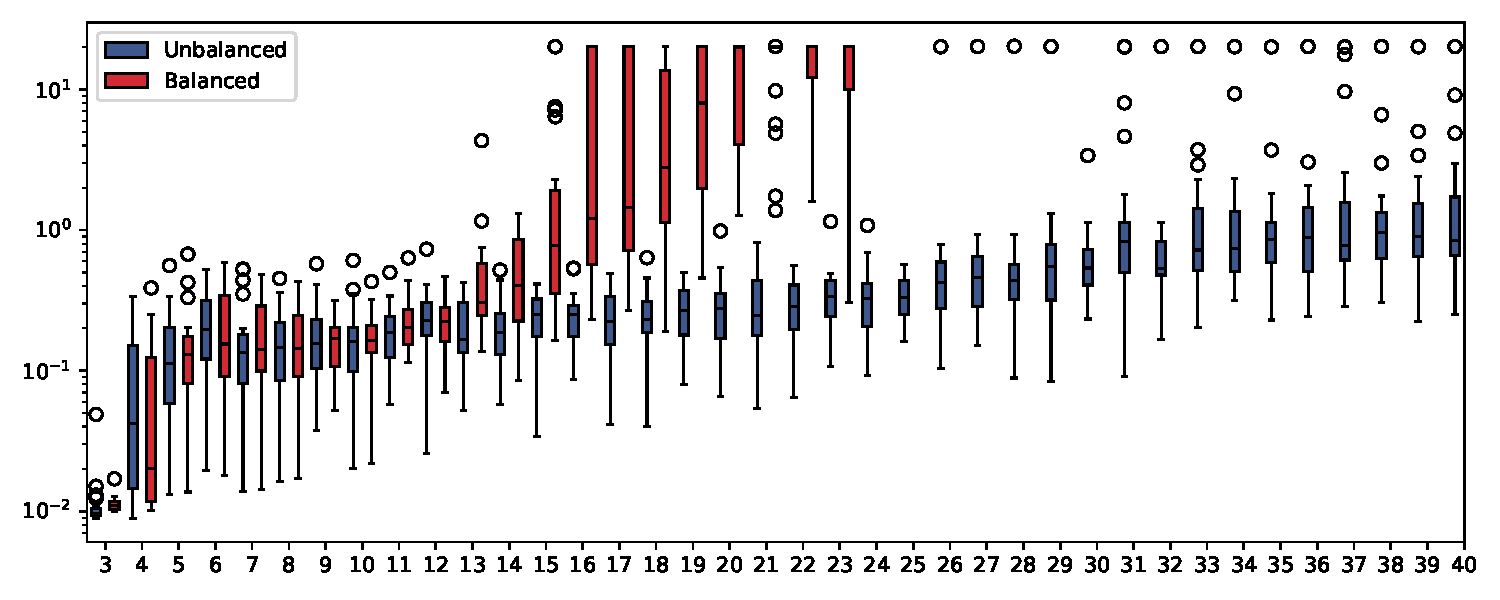
\includegraphics[width=0.8\textwidth]{figures/04_perf.pdf}
    \caption{Time to solve trees of size n (x-axis) with hybrid edges spanning over multiple layers. In seconds (y-axis, log-scale).}
    \label{fig:runtime-multi-hybrid}
\end{figure}
\begin{figure}[H]
    \centering
    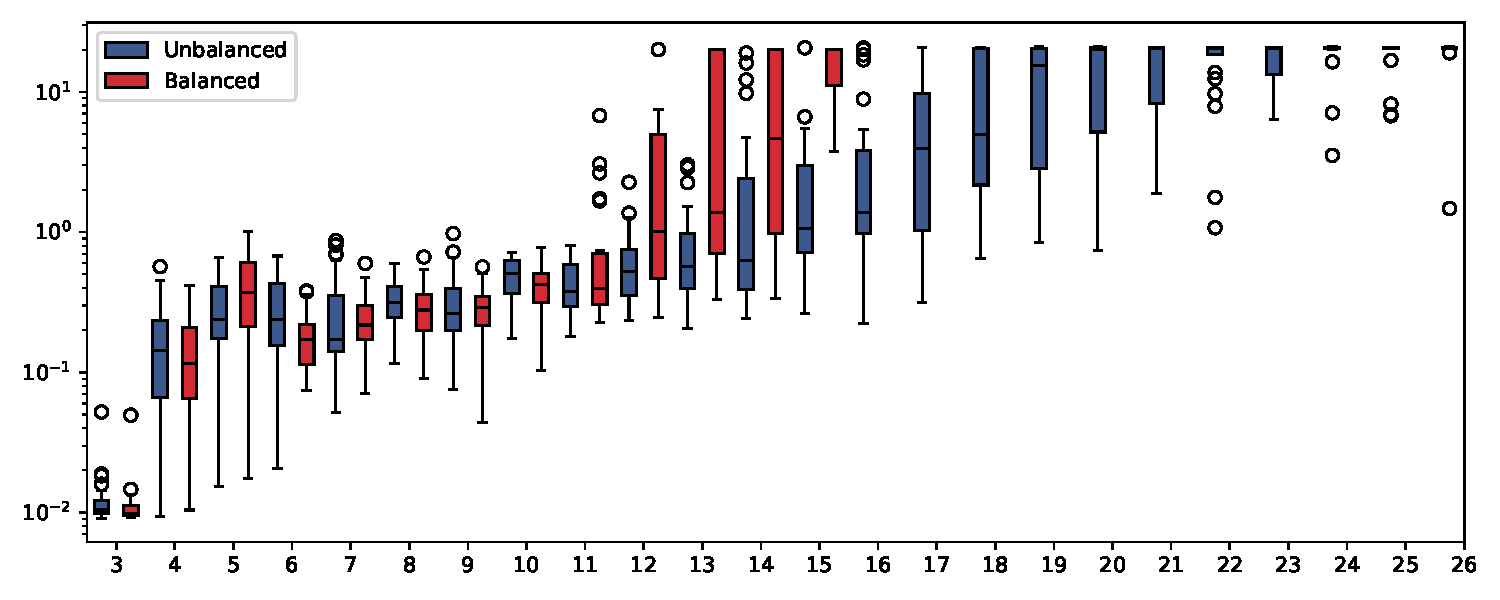
\includegraphics[width=0.8\textwidth]{figures/05_perf.pdf}
    \caption{Time to solve networks of size n (x-axis) in seconds (y-axis, log-scale).}
    \label{fig:runtime-network}
\end{figure}
\newpage
\printbibliography
\end{document}

